\documentclass[xcolor={dvipsnames,svgnames,table}]{beamer}

\input philippe2013_beamer

\title[\'Etudes de fonctions]{{\small Chapitre 2}\\[0.5cm] \textbf{\'Etudes de fonctions}}
\date{}
\author{}

\begin{document}

\begin{frame}
\titlepage
\end{frame}

\section{Fonction $x \mapsto  \abs x$}

\begin{frame}
    \begin{definition}
        Pour tout $x \in \R$, on définit la fonction \alert{valeur absolue} $x \mapsto \abs x$ par :
        \[\abs{x} =
        \left\{\begin{array}{r@{\quad\text{si}\quad}l}
             x & x \geq 0 \\
            -x & x < 0
        \end{array}\right.\]
    \end{definition}

    \begin{Prop}
        Pour tout $x \in \R^*$, la fonction valeur absolue est strictement positive et $\abs 0 = 0$.\par
        Son minimum (la plus petite des images) est donc égal à $0$.
    \end{Prop}
\end{frame}

\begin{frame}
\begin{center}
    \begin{tikzpicture}[>=latex]
        \draw[->] (-5,0) -- (5,0) node[below] {$x$} ;
        \foreach \x in {-4, -3,...,-1} \draw[xshift=\x cm] (0pt,2pt) -- (0pt,-2pt) node[below] {$\x$};
        \foreach \x in {1, 2,...,4} \draw[xshift=\x cm] (0pt,2pt) -- (0pt,-2pt) node[below] {$\x$};
        \draw[->] (0,-1) -- (0,5) node[left] {$y$} ;
        \foreach \y in {1,2,...,4} \draw[yshift=\y cm] (-2pt,0pt) -- (2pt,0pt) node[left=1.5pt] {$\y$};
        \draw (0,0) node[below left] {$0$};
        \draw[blue,thick,domain=-4.75:4.75,samples=200]plot(\x,{abs(\x)}) node[right]{$\abs x$};
        \draw (-2.5,2.5) node[above=-3mm] {\rotatebox{-45}{$\abs x = -x$}};
        \draw (2.5,2.5) node[above=-3mm] {\rotatebox{45}{$\abs x = x$}};
    \end{tikzpicture}
\end{center}
\end{frame}

\begin{frame}
\begin{Prop}
    Sur l'intervalle $\intervalleof{-\infty}{0}$, la fonction valeur absolue est strictement décroissante.\par
    Sur l'intervalle $\intervallefo{0}{+\infty}$, la fonction valeur absolue est strictement croissante.
\end{Prop}

\begin{center}
    \begin{tikzpicture}
        \tkzTabInit[color,espcl=4]%
        {$x$ /1, Variations\\ de $\abs x$ /1.5}%
        {$-\infty$,$0$,$+\infty$}%
        \tkzTabVar[color=red]{ +/ ,-/ $0$,+ /}
    \end{tikzpicture}
\end{center}
\end{frame}

\begin{frame}
    \begin{Prop}
        La représentation graphique de la fonction valeur absolue est symétrique par rapport à l'axe des ordonnées.
    \end{Prop}
\end{frame}

\section{Somme et fonctions composées}

\begin{frame}
On se place dans un repère orthonormé nommé $(O, I, J)$. On considère une fonction $u$ définie sur $\calig D_u$ dont voici la représentation graphique $\calig C_u$ sur un intervalle $A$.

\begin{center}
    \begin{tikzpicture}
        \draw[->] (-1.75,0)--(4,0) node[below] {$x$};
        \draw[->] (0,-0.25)--(0,4) node[left] {$y$};
        \draw (0,0) node[below left] {\small $O$};
        \draw (1,0) node[below=2pt] {\small $I$} node {|};
        \draw (0,1) node[left=2pt] {\small $J$} node {--};
        \draw[color=red,line width=1pt] plot[domain=-1.25:3.6,samples=200] (\x,{cos(deg(\x+0.2))+0.5});
    \end{tikzpicture}
\end{center}

\end{frame}

\subsection{Fonction $t \mapsto u(t) + k$}

\begin{frame}
\uncover<+->{
\begin{Prop}[admise]
    La représentation graphique de la fonction $t \mapsto u(t) + k$ est l'image de $\calig C_u$ par la translation de vecteur $k\times\vect{OJ}$.
\end{Prop}}

\begin{center}
\uncover<+->{
    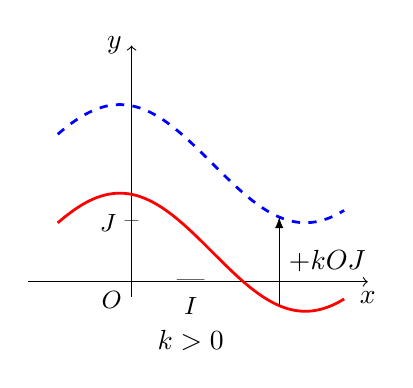
\begin{tikzpicture}[x=0.75cm,y=0.75cm]
        \draw[->] (-1.75,0)--(4,0) node[below] {$x$};
        \draw[->] (0,-0.25)--(0,4) node[left] {$y$};
        \draw (0,0) node[below left] {\small $O$};
        \draw (1,0) node[below=2pt] {\small $I$} node {|};
        \draw (0,1) node[left=2pt] {\small $J$} node {--};
        \draw[color=red,line width=1pt] plot[domain=-1.25:3.6,samples=200] (\x,{cos(deg(\x+0.2))+0.5});
        \draw[color=blue,line width=1pt, dashed] plot[domain=-1.25:3.6,samples=200] (\x,{cos(deg(\x+0.2))+2});
        \draw[->,>=latex,thin] (2.5,{cos(deg(2.5+0.2))+0.5}) -- (2.5,{cos(deg(2.5+0.2))+2}) node[midway,right] {$+k\vect{OJ}$};
        \draw (1,-1) node {$k > 0$};
    \end{tikzpicture}}\quad
    \uncover<+->{
    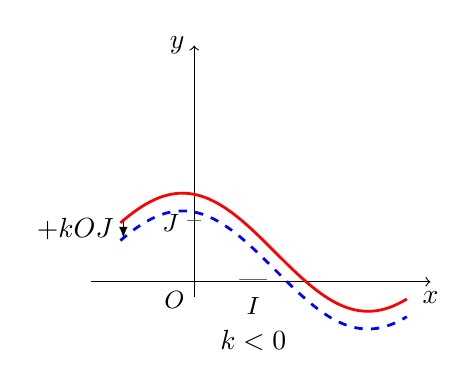
\begin{tikzpicture}[x=0.75cm,y=0.75cm]
        \draw[->] (-1.75,0)--(4,0) node[below] {$x$};
        \draw[->] (0,-0.25)--(0,4) node[left] {$y$};
        \draw (0,0) node[below left] {\small $O$};
        \draw (1,0) node[below=2pt] {\small $I$} node {|};
        \draw (0,1) node[left=2pt] {\small $J$} node {--};
        \draw[color=red,line width=1pt] plot[domain=-1.25:3.6,samples=200] (\x,{cos(deg(\x+0.2))+0.5});
        \draw[color=blue,line width=1pt, dashed] plot[domain=-1.25:3.6,samples=200] (\x,{cos(deg(\x+0.2))+0.2});
        \draw[->,>=latex,thin] (-1.2,{cos(deg(-1.2+0.2))+0.5}) -- (-1.2,{cos(deg(-1.2+0.2))+0.2}) node[midway,left] {$+k\vect{OJ}$};
        \draw (1,-1) node {$k < 0$};
    \end{tikzpicture}}
\end{center}
\end{frame}

\begin{frame}
\begin{Prop}[admise]
    Les fonctions $t \mapsto u(t)$ et $t \mapsto u(t) + k$ ont le même ensemble de définition.
\end{Prop}
\end{frame}

\subsection{Fonction $t \mapsto u(t + \lambda)$}

\begin{frame}
\uncover<+->{
\begin{Prop}[admise]
    La représentation graphique de la fonction $t \mapsto u(t + \lambda)$ est l'image de $\calig C_u$ par la translation de vecteur $-\lambda\times\vect{OI}$.
\end{Prop}
}

\begin{center}
\uncover<+->{
    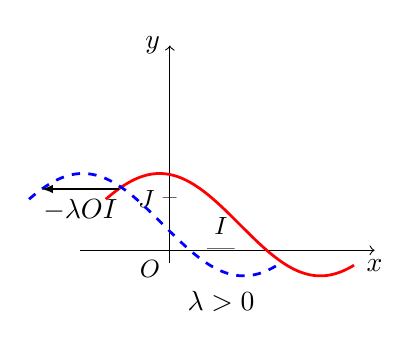
\begin{tikzpicture}[x=0.65cm,y=0.65cm]
        \draw[->] (-1.75,0)--(4,0) node[below] {$x$};
        \draw[->] (0,-0.25)--(0,4) node[left] {$y$};
        \draw (0,0) node[below left] {\small $O$};
        \draw (1,0) node[above=2pt] {\small $I$} node {|};
        \draw (0,1) node[left=2pt] {\small $J$} node {--};
        \draw[color=red,line width=1pt] plot[domain=-1.25:3.6,samples=200] (\x,{cos(deg(\x+0.2))+0.5});
        \draw[color=blue,line width=1pt, dashed] plot[domain=-2.75:2.1,samples=200] (\x,{cos(deg(\x+1.7))+0.5});
        \draw[->,>=latex,thin] (-1,{cos(deg(-1+0.2))+0.5}) -- (-2.5,{cos(deg(-1+0.2))+0.5}) node[midway,below] {$-\lambda\vect{OI}$};
        \draw (1,-1) node {$\lambda > 0$};
    \end{tikzpicture}}\quad\uncover<+->{
    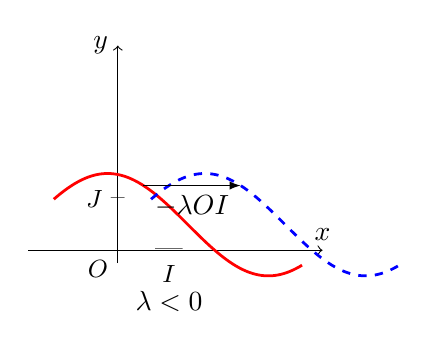
\begin{tikzpicture}[x=0.65cm,y=0.65cm]
        \draw[->] (-1.75,0)--(4,0) node[above] {$x$};
        \draw[->] (0,-0.25)--(0,4) node[left] {$y$};
        \draw (0,0) node[below left] {\small $O$};
        \draw (1,0) node[below=2pt] {\small $I$} node {|};
        \draw (0,1) node[left=2pt] {\small $J$} node {--};
        \draw[color=red,line width=1pt] plot[domain=-1.25:3.6,samples=200] (\x,{cos(deg(\x+0.2))+0.5});
        \draw[color=blue,line width=1pt, dashed] plot[domain=0.65:5.5,samples=200] (\x,{cos(deg(\x-1.7))+0.5});
        \draw[->,>=latex,thin] (0.5,{cos(deg(0.5+0.2))+0.5}) -- (2.4,{cos(deg(0.5+0.2))+0.5}) node[midway,below] {$-\lambda\vect{OI}$};
        \draw (1,-1) node {$\lambda < 0$};
    \end{tikzpicture}}
\end{center}
\end{frame}

\begin{frame}{Remarque}
    L'intervalle de définition de la fonction $u$ subit également une translation. Il faut donc faire attention à cela.
\end{frame}

\begin{frame}
\begin{Example}
\uncover<+->{
    $f \colon x \mapsto \frac 1x$ est défini sur \ldots\par
    Soit $a \in \R$. On pose : $g(x) = f(x + a) = \ldots$ \par
    $\calig D_g = \ldots$
}

\begin{center}
\begin{tikzpicture}[scale=0.5]
\uncover<+->{\begin{scope}
    \clip (-4.5,-4.5) rectangle (4.5,4.5);
        \draw[->] (-4,0)--(4,0) node[below] {$x$};
        \draw[->] (0,-4)--(0,4) node[left] {$y$};
        \draw (0,0) node[below left] {\small $O$};
        \draw (1,0) node[below=2pt] {\small $I$} node {|};
        \draw (0,1) node[left=2pt] {\small $J$} node {--};
    \draw[smooth,samples=200,domain=-4:-0.1] plot(\x,{1/\x});
    \draw[smooth,samples=200,domain=0.1:4] plot(\x,{1/\x});
\end{scope}}
\uncover<+->{
\begin{scope}[xshift=10cm]
    \clip (-4.5,-4.5) rectangle (4.5,4.5);
        \draw[->] (-4,0)--(4,0) node[below] {$x$};
        \draw[->] (0,-4)--(0,4) node[left] {$y$};
        \draw (0,0) node[below left] {\small $O$};
        \draw (1,0) node[above=2pt] {\small $I$} node {|};
        \draw (0,1) node[left=2pt] {\small $J$} node {--};
    \draw[smooth,samples=200,domain=-4:1.4] plot(\x,{1/(\x-1.5)});
    \draw[smooth,samples=200,domain=1.6:4] plot(\x,{1/(\x-1.5)});
    \draw[dashed, blue] (1.5,-4.5) -- (1.5,4.5) node[below right=-2pt,midway] {\scriptsize$-a$} node[midway]{$\times$};
\end{scope}}
\end{tikzpicture}
\end{center}
\end{Example}
\end{frame}

\subsection{Fonction $t \mapsto \abs{u(t)}$}

\begin{frame}
\uncover<+->{
\begin{Prop}[admise]
    Deux cas se présentent :
    \begin{enumerate}
        \item Sur la réunion de tous les intervalles où la fonction $u$ est positive, alors $\calig C_u$ est confondue avec la courbe de $\abs u$.
        \item Sinon, la courbe représentative de la fonction $\abs u$ est l'image de $\calig C_u$ par la symétrie d'axe $(OI)$.
    \end{enumerate}
\end{Prop}
}
\uncover<+->{
\begin{center}
    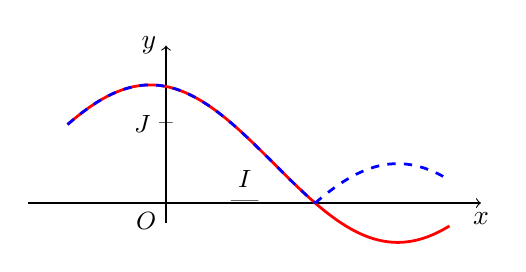
\begin{tikzpicture}
        \draw[->] (-1.75,0)--(4,0) node[below] {$x$};
        \draw[->] (0,-0.25)--(0,2) node[left] {$y$};
        \draw (0,0) node[below left] {\small $O$};
        \draw (1,0) node[above=2pt] {\small $I$} node {|};
        \draw (0,1) node[left=2pt] {\small $J$} node {--};
        \draw[color=red,line width=1pt] plot[domain=-1.25:3.6,samples=200] (\x,{cos(deg(\x+0.2))+0.5});
        \uncover<+->{\draw[color=blue,line width=1pt, dashed] plot[domain=-1.25:{rad(acos(-0.5))-0.2},samples=200] (\x,{cos(deg(\x+0.2))+0.5});
        \draw[color=blue,line width=1pt, dashed] plot[domain={rad(acos(-0.5))-0.2}:3.6,samples=200] (\x,{-cos(deg(\x+0.2))-0.5});}
    \end{tikzpicture}
\end{center}}
\end{frame}

\begin{frame}
\begin{Prop}[admise]
    Les fonctions $t\mapsto u(t)$ et $t\mapsto\abs{u(t)}$ ont le même domaine de définition.
\end{Prop}
\end{frame}


\end{document} 